\begin{refsection}

\chapter{Pb--Pb and Th--Pb}
\label{ch:ThPbPb-R}

\section{Pb--Pb}\label{sec:PbPb-R}

\noindent\begin{minipage}[t]{.3\linewidth}
\strut\vspace*{-\baselineskip}\newline
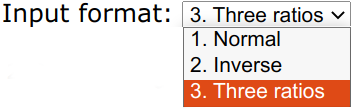
\includegraphics[width=\linewidth]{../figures/PbPbFormats.png}
\end{minipage}
\begin{minipage}[t]{.7\textwidth}
  \texttt{IsoplotR} accommodates three Pb--Pb formats. See
  Section~\ref{sec:PbPb} for details.
\end{minipage}

\begin{console}
PbPb <- read.data('PbPb3.csv',method='Pb-Pb',format=3)
\end{console}

\noindent which returns a list with items \texttt{format} and
\texttt{x} containing the input format and isotopic ratio data,
respectively.\\

\noindent\begin{minipage}[t]{.15\linewidth}
\strut\vspace*{-\baselineskip}\newline
\includegraphics[width=\linewidth]{../figures/PbPbPlotdevices.png}\\
\end{minipage}
\begin{minipage}[t]{.85\textwidth}
  Pb--Pb data can be visualised on five different plot devices.
  Additionally, the single aliquot age estimates can also be reported
  in a downloadable data table.
\end{minipage}

\noindent\begin{minipage}[t]{.6\linewidth}
\strut\vspace*{-\baselineskip}\newline
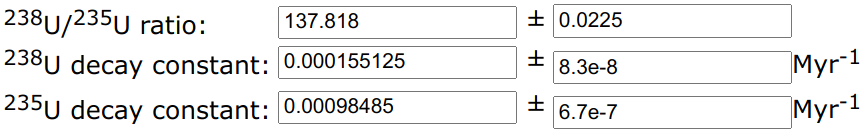
\includegraphics[width=\linewidth]{../figures/PbPbLambda.png}
\end{minipage}
\begin{minipage}[t]{.4\linewidth}
  The default \textsuperscript{238}U/\textsuperscript{235}U ratio is
  given by \citet{hiess2012}, and the U decay constants by
  \citet{jaffey1971}. These values can be changed here.
\end{minipage}

\begin{script}
# use the Steiger and Jaeger (1977) value with zero uncertainty
settings('iratio','U238U235',137.88,0)
# use the Schoene et al. (2006) value and uncertainty
settings('lambda','U238',0.000154993,0.00000013) 
\end{script}

\section{Pb--Pb isochrons}\label{sec:PbPb-isochrons-R}

\begin{enumerate}

\item \texttt{IsoplotR} offers the same three options to deal with the
  scatter of the data around the best-fit isochron line as the generic
  regression function of Section~\ref{sec:OtherRegression}.

\noindent\begin{minipage}[t]{.45\linewidth}
\strut\vspace*{-\baselineskip}\newline
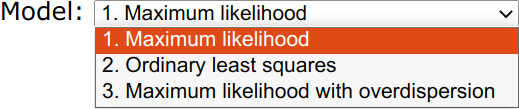
\includegraphics[width=\linewidth]{../figures/PbPbIsochronModels.png}
\end{minipage}
\begin{minipage}[t]{.55\linewidth}
  These three models represent three different ways to capture any
  excess dispersion of the data w.r.t. the analytical uncertainties
  (Figure~\ref{fig:isochronMSWD}).
\end{minipage}

\begin{console}
isochron(PbPb,model=1)
\end{console}

\item Data can be fitted using conventional
  (\textsuperscript{207}Pb/\textsuperscript{204}Pb
  vs. \textsuperscript{206}Pb/\textsuperscript{204}Pb) or inverse
  (\textsuperscript{207}Pb/\textsuperscript{206}Pb
  vs. \textsuperscript{204}Pb/\textsuperscript{206}Pb) isochrons
  (Section~\ref{sec:inverseIsochrons}).

  \noindent\begin{minipage}[t]{.22\linewidth}
\strut\vspace*{-\baselineskip}\newline

\includegraphics[width=\linewidth]{../figures/PbPbisochronInverse.png}
\end{minipage}
\begin{minipage}[t]{.78\linewidth}
  These two types of isochron yield similar ages provided that the
  uncertainties are relatively small compared to the isotopic ratio
  values.
\end{minipage}

\begin{console}
isochron(PbPb,inverse=TRUE)
\end{console}

\item As discussed in Section~\ref{sec:SKgrowth}, the mantle evolution
  model of \citet{stacey1975} can be included with the isochron plot.

\noindent\begin{minipage}[t]{.45\linewidth}
\strut\vspace*{-\baselineskip}\newline

\includegraphics[width=\linewidth]{../figures/PbPbIsochronSKcurve.png}
\end{minipage}
\begin{minipage}[t]{.55\linewidth}
  Any intersections of the isochron with the mantle evolution curve
  are reported in the plot legend.
\end{minipage}

The Stacey-Kramers curve may not be easy to spot for very radiogenic
samples. So here is an example of some whole rock Pb--Pb analyses that
are relatively poor in uranium \citep{kamber1998}:

\begin{script}
PbPb2 <- read.data('Kamber.csv',method='Pb-Pb',format=1)
isochron(PbPb2,growth=TRUE)
\end{script}

\item The appearance and numerical behaviour of Pb--Pb isochrons can
  be modified using similar options as the U--Pb isochrons of
  Section~\ref{sec:UPb-isochron-R}, and as the general regression of
  Section~\ref{sec:OtherRegression}.

\noindent\begin{minipage}[t]{.4\linewidth}
\strut\vspace*{-\baselineskip}\newline
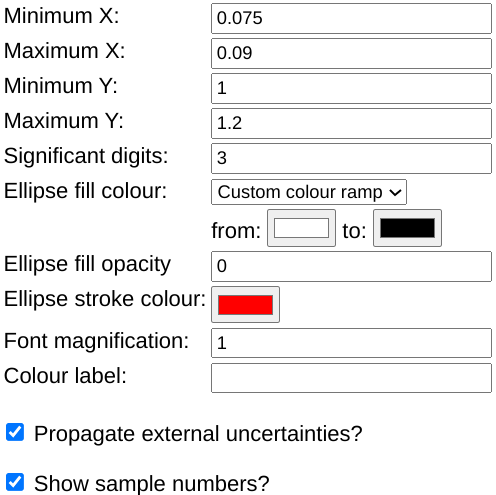
\includegraphics[width=\linewidth]{../figures/PbPbIsochronOtherOptions.png}
\end{minipage}
\begin{minipage}[t]{.6\linewidth}
  Tick the checkbox to propagate decay constant uncertainties
  (\texttt{exterr}) and label the error ellipses with the row numbers
  of the input data (\texttt{show.numbers}). Use the textboxes to set
  the axis limits (\texttt{xlim} and \texttt{ylim}), significance
  level (\texttt{alpha}), significant digits (\texttt{sigdig}), the
  fill and stroke colour of the error ellipses (\texttt{ellipse.fill}
  and \texttt{ellipse.stroke}), font size (\texttt{cex}) and colour
  legend (\texttt{levels} and \texttt{clabel}).
\end{minipage}

\begin{script}
isochron(PbPb,exterr=TRUE,show.numbers=TRUE,xlim=c(0,0.03),ylim=c(0,0.75),
         alpha=0.01,sigdig=3,ellipse.fill=NA,ellipse.stroke="red")
\end{script}
  
\end{enumerate}

\section{Pb--Pb ages}\label{sec:PbPbAges}

Although, as discussed in Section~\ref{sec:ThPbPbradial}, Pb--Pb ages
are usually calculated by isochron regression, it is also possible to
obtain the ages of the individual aliquots. Once these have been
calculated, it is then straightforward to turn them into the radial,
weighted mean, KDE and CAD plots. Thus, it is useful to introduce
\texttt{IsoplotR}'s age calculation function before discussing the
aforementioned plots.

\begin{enumerate}

\item In contrast with the U--Pb method, in which common-Pb correction
  often does not affect the age much, this correction is crucial for
  single grain Pb--Pb dating.
  
\noindent\begin{minipage}[t]{.35\linewidth}
\strut\vspace*{-\baselineskip}\newline
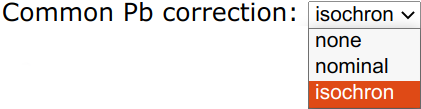
\includegraphics[width=\linewidth]{../figures/PbPbRadialPb0.png}
\end{minipage}
\begin{minipage}[t]{.65\linewidth}
  In contrast with the U--Pb data of Section~\ref{sec:UPbRadial}, the
  common Pb correction of Pb--Pb data is limited to two options:
  nominal and isochron. These implement the two procedures shown in
  Figure~\ref{fig:ThPbSingleGrain}.
\end{minipage}

By default the CLI version of the \texttt{age()} function returns the
isochron age. To produce a table of single-aliquot ages, the optional
\texttt{isochron} argument must be set to \texttt{FALSE}:

\begin{console}
age(PbPb,isochron=FALSE,common.Pb=2)
\end{console}

\item Nominal common Pb correction of the Pb--Pb data proceeds like
  the nominal common Pb correction of U--Pb data formats 4--6
  (Section~\ref{sec:general}).

\noindent\begin{minipage}[t]{.4\linewidth}
\strut\vspace*{-\baselineskip}\newline
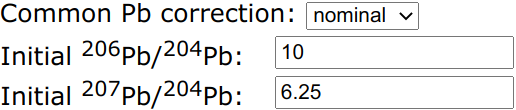
\includegraphics[width=\linewidth]{../figures/PbPbnominalPb0.png}
\end{minipage}
\begin{minipage}[t]{.6\linewidth}
  The nominal \textsuperscript{207}Pb/\textsuperscript{204}Pb and
  \textsuperscript{206}Pb/\textsuperscript{204}Pb ratios in this
  example correspond to a
  \textsuperscript{207}Pb/\textsuperscript{206}Pb ratio of 0.625,
  which equals the y-intercept of the inverse isochron.
\end{minipage}

\begin{console}
settings('iratio','Pb207Pb204',6.25)
settings('iratio','Pb206Pb204',10)
age(PbPb,isochron=FALSE,common.Pb=1)
\end{console}

\item The systematic uncertainty of the decay constants can be added
  to the single grain age estimates by ticking the corresponding box.

\noindent\begin{minipage}[t]{.38\linewidth}
\strut\vspace*{-\baselineskip}\newline

\includegraphics[width=\linewidth]{../figures/exterr.png}
\end{minipage}
\begin{minipage}[t]{.62\linewidth}
Be aware that this will introduce error correlations between the
different aliquots, which are not reported in the data table!
\end{minipage}

\begin{console}
age(PbPb,isochron=FALSE,common.Pb=2,exterr=TRUE)
\end{console}
  
\item The uncertainty associated with the common Pb correction is
  neither a purely systematic nor a purely random uncertainty.

\noindent\begin{minipage}[t]{.5\linewidth}
\strut\vspace*{-\baselineskip}\newline

\includegraphics[width=\linewidth]{../figures/projerr.png}
\end{minipage}
\begin{minipage}[t]{.5\linewidth}
  Including the common-Pb uncertainty may significantly increase the
  single grain age errors whilst causing strong error correlations,
  which are not reported in the output table.
\end{minipage}

\begin{console}
age(PbPb,isochron=FALSE,common.Pb=2,exterr=TRUE,projerr=TRUE)
\end{console}

\end{enumerate}

\section{Th--Pb}\label{sec:ThPb-R}

\noindent\begin{minipage}[t]{.3\linewidth}
\strut\vspace*{-\baselineskip}\newline
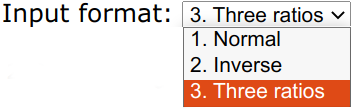
\includegraphics[width=\linewidth]{../figures/PbPbFormats.png}
\end{minipage}
\noindent\begin{minipage}[t]{.15\linewidth}
\strut\vspace*{-\baselineskip}\newline
\includegraphics[width=\linewidth]{../figures/PbPbPlotdevices.png}\\
\end{minipage}
\begin{minipage}[t]{.55\textwidth}
  \texttt{IsoplotR} accommodates three Th--Pb formats (see
  Section~\ref{sec:ThPb} for details), which can be analysed by the
  same six functions as the Pb--Pb data (Section~\ref{sec:PbPb-R}).
\end{minipage}

\begin{console}
ThPb <- read.data('ThPb2.csv',method='Th-Pb',format=2)
\end{console}

\noindent which returns a list with items \texttt{format} and
\texttt{x} containing the input format and isotopic ratio data,
respectively.\\

\noindent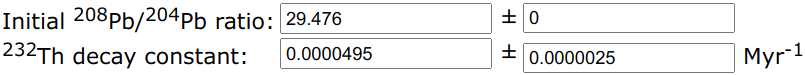
\includegraphics[width=.7\linewidth]{../figures/ThPbLambda.png}\\
\noindent The default values for the initial
\textsuperscript{208}Pb/\textsuperscript{204}Pb ratio and its standard
error are taken from \citet{stacey1975}. These values are hidden from
the \texttt{isochron} function. The default Th decay constant is given
by \citet{leroux1963}.

\begin{script}
# round the inherited 208Pb/204Pb ratio to 30 +/- 0
settings('iratio','Pb208Pb204',30,0) 
# round the 232Th decay constant to 0.00005 +/- 0.000003
settings('lambda','Th232',0.00005,0.000003) 
\end{script}

\section{Th--Pb isochrons}\label{sec:ThPb-isochrons-R}

Isochron regression proceeds in exactly the same fashion as the
generic regression function of Section~\ref{sec:OtherRegression},
apart from just two small geochronology-specific differences:\\

\noindent\begin{minipage}[t]{.35\linewidth}
\strut\vspace*{-\baselineskip}\newline

\includegraphics[width=\linewidth]{../figures/ThPbInverseExterr.png}
\end{minipage}
\begin{minipage}[t]{.65\linewidth}
Both conventional and inverse isochrons are available, and the
analytical uncertainty of the resulting ages may be augmented by the
decay constant uncertainties.\\
\end{minipage}

\begin{console}
isochron(ThPb,inverse=TRUE,exterr=FALSE)
\end{console}

The remaining isochron settings are identical to the those of the
generic regression function of Section~\ref{sec:OtherRegression}. For
example, the following code snippet creates an inverse Th--Pb isochron
with empty blue error ellipses numbered by aliquot:

\begin{script}
isochron(ThPb,inverse=TRUE,show.numbers=TRUE,
         ellipse.fill=NA,ellipse.stroke=rgb(0,0,1,0.5))
\end{script}

\section{Th--Pb ages}\label{sec:ThPbAges}

Th--Pb age calculation can either be done

\begin{enumerate}

\item by projection along the inverse isochron
  (Figure~\ref{fig:ThPbSingleGrain}):

\noindent
\includegraphics[width=.75\linewidth]{../figures/ThPbAgei2i.png}

\begin{console}
age(ThPb,isochron=FALSE,i2i=TRUE)
\end{console}

\noindent where the \texttt{i2i} argument stands for
`intercept-to-initial ratio';

\item or using a nominal common Pb correction:

\noindent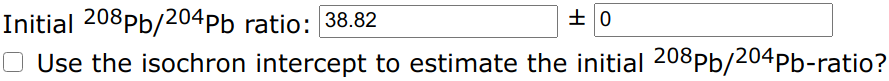
\includegraphics[width=.75\linewidth]{../figures/ThPbAgePb0.png}

\noindent which, at the CLI, is specified via the \texttt{settings()} function:

\begin{script}
settings('iratio','Pb208Pb204',38.82)
age(ThPb,isochron=FALSE,i2i=FALSE)
\end{script}

\item The systematic uncertainties associated with the decay constant
  errors and common Pb correction can be added to the single grain age
  estimates.

\noindent\begin{minipage}[t]{.5\linewidth}
\strut\vspace*{-\baselineskip}\newline

\includegraphics[width=\linewidth]{../figures/projexterr.png}
\end{minipage}
\begin{minipage}[t]{.5\linewidth}
  This will expand the uncertainties and produce error correlations
  between the different aliquots, which are \emph{not} reported in the
  data table.
\end{minipage}
  
\end{enumerate}

\section{Radial, weighted mean, KDE and CAD plots}
\label{sec:ThPbPbOtherPlots}

The settings for the radial, weighted mean, KDE and CAD plots combine
the generic settings for those graphical devices
(Sections~\ref{sec:OtherRadial}--\ref{sec:OtherCAD}) with the settings
for the age calculator (Sections~\ref{sec:PbPbAges} and
\ref{sec:ThPbAges}).\\

\noindent\begin{minipage}[t]{.45\linewidth}
\strut\vspace*{-\baselineskip}\newline
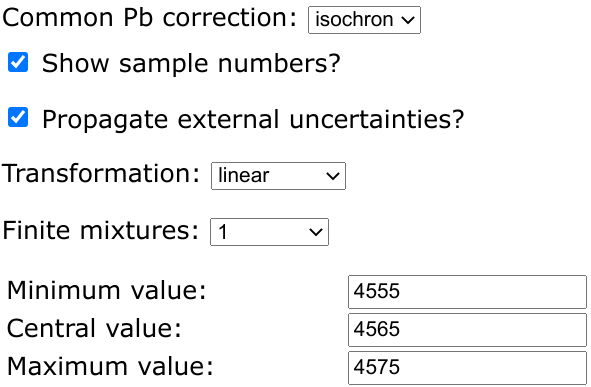
\includegraphics[width=\linewidth]{../figures/PbPbRadialOptions.png}
\end{minipage}
\begin{minipage}[t]{.55\linewidth}
  For example, here are shown the GUI settings for a radial plot of
  numbered Pb--Pb data, which is plotted on a linear scale that
  stretches from 4555 to 4575~Ma and is centred around 4565~Ma. Single
  grain ages are corrected using the isochron-based common Pb
  composition, and a single age component is fitted to them. The
  standard errors of the central age and the single component age
  include decay constant uncertainties.
\end{minipage}

\begin{script}
radialplot(PbPb,show.numbers=TRUE,exterr=TRUE,transformation='linear',
           k=1,from=4555,to=4575,z0=4565)
\end{script}

Note that whilst it is possible to propagate the systematic error
associated with the decay constant uncertainties, \texttt{IsoplotR}
currently \textbf{does not provide a means to propagate the
  uncertainty of the common Pb correction} (i.e., the \texttt{projerr}
argument in the \texttt{age()} function). This uncertainty is neither
a purely systematic nor a purely random uncertainty and cannot easily
be propagated with conventional geochronological data processing
algorithms. This caveat is especially pertinent when the common Pb
correction has been determined by isochron regression. You may note
that the uncertainties of the central age are usually much smaller
than those of the isochron. In this case the isochron errors are more
meaningful, and the radial plot should just be used to inspect the
residuals of the data around the isochron.\\

The same caveat applies to the weighted mean plot. The KDE and CAD
functions are, of course, immune to this problem because they are not
associated with any numerical output. These functions therefore work
exactly as the generic versions of Chapter~\ref{ch:generic-R}, with
the only difference being the common Pb correction.\\

\noindent CLI examples:

\begin{enumerate}

\item The weighted mean using a nominal common Pb correction with
  \textsuperscript{206}Pb/\textsuperscript{204}Pb = 9.15 and
  \textsuperscript{207}Pb/\textsuperscript{204}Pb = 10.23; applying
  the random effects model and plotting the ranked ages:
  
\begin{script}
settings('iratio','Pb206Pb204',9.15)
settings('iratio','Pb207Pb204',10.23)
weightedmean(PbPb,common.Pb=1,random.effects=TRUE,ranked=TRUE)
\end{script}

\item An orange KDE without histogram or rug plot, using an
  isochron-based common Pb correction, with a 20~Myr bandwidth and
  axis limits from 4500 to 4650~Ma:

\begin{script}
kde(PbPb,kde.col='orange',rug=FALSE,show.hist=FALSE,
    common.Pb=2,bw=20,from=4500,to=4650)
\end{script}

\item A CAD with without vertical lines and steps marked by `x':

\begin{console}
cad(PbPb,verticals=TRUE,pch='x')
\end{console}

\item A radial plot of Th--Pb isochron residuals:

\begin{console}
radialplot(ThPb,i2i=TRUE)
\end{console}

\noindent where the central age is marked by an asterisk in the title
of the radial plot to indicate the circularity of using an
isochron-based common Pb correction to compute a central age.

\end{enumerate}

\printbibliography[heading=subbibliography]

\end{refsection}
